%% LyX 2.2.3 created this file.  For more info, see http://www.lyx.org/.
%% Do not edit unless you really know what you are doing.
\documentclass[english,12pt]{article}
\usepackage[T1]{fontenc}
\usepackage[latin9]{inputenc}
\usepackage{float}
\usepackage{mathtools}
\usepackage{amsmath}
\usepackage{amsthm}
\usepackage{amssymb}
\usepackage{graphicx}

\makeatletter
%%%%%%%%%%%%%%%%%%%%%%%%%%%%%% Textclass specific LaTeX commands.
\theoremstyle{plain}
\newtheorem{thm}{\protect\theoremname}[section]
\theoremstyle{plain}
\newtheorem{prop}[thm]{\protect\propositionname}
\ifx\proof\undefined
\newenvironment{proof}[1][\protect\proofname]{\par
\normalfont\topsep6\p@\@plus6\p@\relax
\trivlist
\itemindent\parindent
\item[\hskip\labelsep\scshape #1]\ignorespaces
}{%
\endtrivlist\@endpefalse
}
\providecommand{\proofname}{Proof}
\fi

%%%%%%%%%%%%%%%%%%%%%%%%%%%%%% User specified LaTeX commands.
\usepackage[margin=1in]{geometry}

\makeatother

\usepackage{babel}
\providecommand{\propositionname}{Proposition}
\providecommand{\theoremname}{Theorem}

\begin{document}

\title{Math 525: Lecture 11}

\date{February 8, 2018}
\maketitle

\section{Laws of large numbers}

Intuitively, we know that
\[
\frac{\text{number of successes in }n\text{ independent trials}}{n}\rightarrow\mathbb{P}(\text{success})
\]
as $n\rightarrow\infty$. This lecture aims to prove this.

Let's first restate the above in terms of random variables. Let $X_{i}$
be the random variable whose value is $1$ if the $i$-th trial is
a success and whose value is $0$ otherwise. In other words,
\[
X_{i}=I_{\{i\text{-th trial is a success}\}}.
\]
Since the trials are independent, we must assume that $X_{i}$ is
independent of $X_{j}$ for $i\neq j$. Then, the number of successes
in the first $n$ trials is simply
\[
X_{1}+\cdots+X_{n}
\]
Using this notation, our first claim becomes
\[
\frac{1}{n}\left(X_{1}+\cdots+X_{n}\right)\rightarrow\mathbb{E}[X_{1}],
\]
which is a statement about sums of random variables converging to
the mean $\mu=\mathbb{E}[X_{1}]$ (we are purposely vague as to the
type of convergence for the time being). Defining $X_{i}^{\prime}=X_{i}-\mu$
and using the claim above, note that
\[
\frac{1}{n}\left(X_{1}+\cdots+X_{n}\right)-\mu=\frac{1}{n}\left(X_{1}-\mu+\cdots+X_{n}-\mu\right)=\frac{1}{n}\left(X_{1}^{\prime}+\cdots+X_{n}^{\prime}\right)\rightarrow0
\]
and hence we can simply focus on the mean-zero case.
\begin{prop}[Weak law of large numbers]
 Let $(X_{n})_{n}$ be an i.i.d. sequence of square integrable, mean
zero random variables. Then,
\[
\frac{1}{n}\left(X_{1}+\cdots+X_{n}\right)\rightarrow0
\]
in probability.
\end{prop}
For the remainder of this lecture, we will use the notation $S_{n}=X_{1}+\cdots+X_{n}$.
\begin{proof}
First, note that
\[
\mathbb{E}\left[\left(\frac{1}{n}S_{n}\right)^{2}\right]=\frac{1}{n^{2}}\mathbb{E}\left[X_{1}X_{1}+X_{1}X_{2}+\cdots+X_{1}X_{n}+\cdots+X_{n}X_{n}\right].
\]
By independence, $\mathbb{E}[X_{i}X_{j}]=0$ whenever $i\neq j$.
Therefore, the above becomes
\[
\mathbb{E}\left[\left(\frac{1}{n}S_{n}\right)^{2}\right]=\frac{1}{n^{2}}\left(\mathbb{E}\left[X_{1}^{2}\right]+\cdots+\mathbb{E}\left[X_{n}^{2}\right]\right)=\frac{n\sigma^{2}}{n^{2}}=\frac{\sigma^{2}}{n}
\]
where we have used $\sigma^{2}=\mathbb{E}[X_{1}^{2}]$. By Markov's/Chebyshev's
inequality,
\[
\mathbb{P}\left\{ \frac{1}{n}\left|S_{n}\right|\geq\epsilon\right\} \leq\frac{1}{\epsilon^{2}}\frac{\sigma^{2}}{n}\rightarrow0.\qedhere
\]
\end{proof}
The above is called a ``weak law'' since convergence is in probability.
There are various ``strong laws'' which guarantee convergence a.e.
Here's one:
\begin{prop}[Cantelli's strong law of large numbers]
Let $(X_{n})_{n}$ be an i.i.d. sequence of mean zero random variables,
with $X_{1}^{4}$ integrable. Then,
\[
\frac{1}{n}S_{n}\rightarrow0\text{ a.s.}
\]
\end{prop}
\begin{proof}
Note that
\[
\mathbb{E}\left[\left(\frac{1}{n}S_{n}\right)^{4}\right]=\frac{1}{n^{4}}\sum_{1\leq i,j,k,\ell\leq n}\mathbb{E}\left[X_{i}X_{j}X_{k}X_{\ell}\right].
\]
Using the same arguments as in the proof of the weak law of large
numbers, note that the only terms that do not have expectation of
zero in the sum are of the form $X_{i}^{4}$ and $X_{i}^{2}X_{j}^{2}$
for $i\neq j$. That is,
\[
\mathbb{E}\left[\left(\frac{1}{n}S_{n}\right)^{4}\right]=\frac{1}{n^{4}}\sum_{i=1}^{n}\left(\mathbb{E}\left[X_{i}^{4}\right]+\sum_{\substack{j=1\\
j\neq i
}
}^{n}\mathbb{E}\left[X_{i}^{2}X_{j}^{2}\right]\right).
\]
Let $\mathbb{E}[X_{1}^{4}]=M$. Then,
\[
\mathbb{E}\left[X_{i}^{2}X_{j}^{2}\right]\leq\sqrt{\mathbb{E}\left[X_{i}^{4}\right]\mathbb{E}\left[X_{j}^{4}\right]}\leq\sqrt{M\cdot M}=M
\]
so that
\[
\mathbb{E}\left[\left(\frac{1}{n}S_{n}\right)^{4}\right]\leq\frac{1}{n^{4}}\sum_{i=1}^{n}\left(M+\left(n-1\right)M\right)=\frac{M+\left(n-1\right)M}{n^{3}}=\frac{M}{n^{2}}.
\]
Chebyshev's inequality tells us
\[
\mathbb{P}\left\{ \frac{\left|S_{n}\right|}{n}\geq\lambda\right\} \leq\frac{1}{\lambda^{4}}\frac{M}{n^{2}}.
\]
Pick $\lambda=n^{-1/8}$ and define
\[
\Lambda_{n}=\left\{ \frac{\left|S_{n}\right|}{n}\geq\frac{1}{n^{1/8}}\right\} 
\]
so that
\[
\sum_{n}\mathbb{P}(\Lambda_{n})\leq\sum_{n}\frac{M}{n^{3/2}}<\infty.
\]
Now, the Borel-Cantelli lemma tells us
\[
1-\mathbb{P}(\liminf_{n}\Lambda_{n}^{c})=\mathbb{P}(\limsup_{n}\Lambda_{n})=0.
\]
In other words, for all $\omega\in\liminf_{n}\Lambda_{n}^{c}$, we
can find $N(\omega)$ such that for all $n\geq N(\omega)$, 
\[
\frac{\left|S_{n}\right|}{n}<\frac{1}{n^{1/8}}.
\]
That is, $S_{n}/n$ converges to zero a.s.
\end{proof}

\section{Empirical distribution}

Let $(X_{n})_{n}$ be a sequence of i.i.d. random variables and define
its \emph{empirical distribution} by
\[
F_{n}(x)=\frac{1}{n}\left|\left\{ j\leq n\colon X_{j}\leq x\right\} \right|.
\]
In other words, $F_{n}(x)$ counts exactly how many of the first $n$
random variables are at most $x$. Unlike the distribution function
$F$, $F_{n}(x)$ is itself a random variable. Sometimes, we might
write
\[
(F_{n}(x))(\omega)
\]
to stress this fact.
\begin{prop}
Let $(X_{n})_{n}$ be a sequence of i.i.d. random variables with distribution
function $F$ and empirical distribution $F_{n}$. Then,
\[
F_{n}\rightarrow F\text{ a.s. }
\]
\end{prop}
Actually, $F_{n}\rightarrow F$ in a stronger sense than pointwise,
but we will not prove that.

\begin{figure}[H]
\begin{centering}
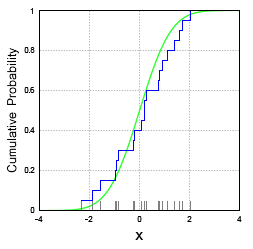
\includegraphics[height=3in]{empirical}
\par\end{centering}
\caption{Empirical distribution converging to the \emph{actual} distribution}
\end{figure}
\begin{proof}
Let $(U_{n})_{n}$ be a sequence i.i.d. $U[0,1]$ random variables
with empirical distribution $F_{n}^{0}$. Let $F^{0}$ be the \emph{actual}
distribution function of $U_{1}$. Now, fix $x\in[0,1]$ and let $Y_{i}=I_{\{U_{i}\leq x\}}$.
Note that $\mathbb{E}[Y_{i}]=\mathbb{P}(U_{i}\leq x)=x$. Then,
\[
\frac{1}{n}\sum_{i=1}^{n}Y_{i}=F_{n}^{0}(x).
\]
Since $\mathbb{E}[Y_{i}^{4}]$ is a constant independent of $i$,
Cantelli's strong law of large numbers tells us
\[
F_{n}^{0}(x)\rightarrow F^{0}(x)\text{ a.s.}
\]

It remains to extend this to general random variables. We will not
do the most general case here and instead focus on the case when $F$
is bijective. Without loss of generality, $X_{n}=F^{-1}(U_{n})$.
Therefore,
\begin{multline*}
F_{n}(x)=\frac{1}{n}\left|\left\{ j\leq n\colon X_{j}\leq x\right\} \right|=\frac{1}{n}\left|\left\{ j\leq n\colon F^{-1}(U_{j})\leq x\right\} \right|=\frac{1}{n}\left|\left\{ j\leq n\colon U_{j}\leq F(x)\right\} \right|\\
=F_{n}^{0}(F(x)).
\end{multline*}
Since $F^{0}(x)=x$ whenever $x\in[0,1]$,
\[
\left|F(x)-F_{n}(x)\right|=\left|F^{0}(F(x))-F_{n}^{0}(F(x))\right|\rightarrow0\text{ a.s.},
\]
as desired.
\end{proof}

\section{Bernstein polynomials}

In a real analysis course, you might have learned that the set of
all polynomials on $[0,1]$, call it $\mathcal{P}[0,1]$, is dense
in $C[0,1]$, the set of all continuous real-valued functions from
$[0,1]$. This is called the \emph{Stone-Weirestrass theorem}. We
now give a constructive proof of this fact, using probability theory!

\begin{figure}[H]
\begin{centering}
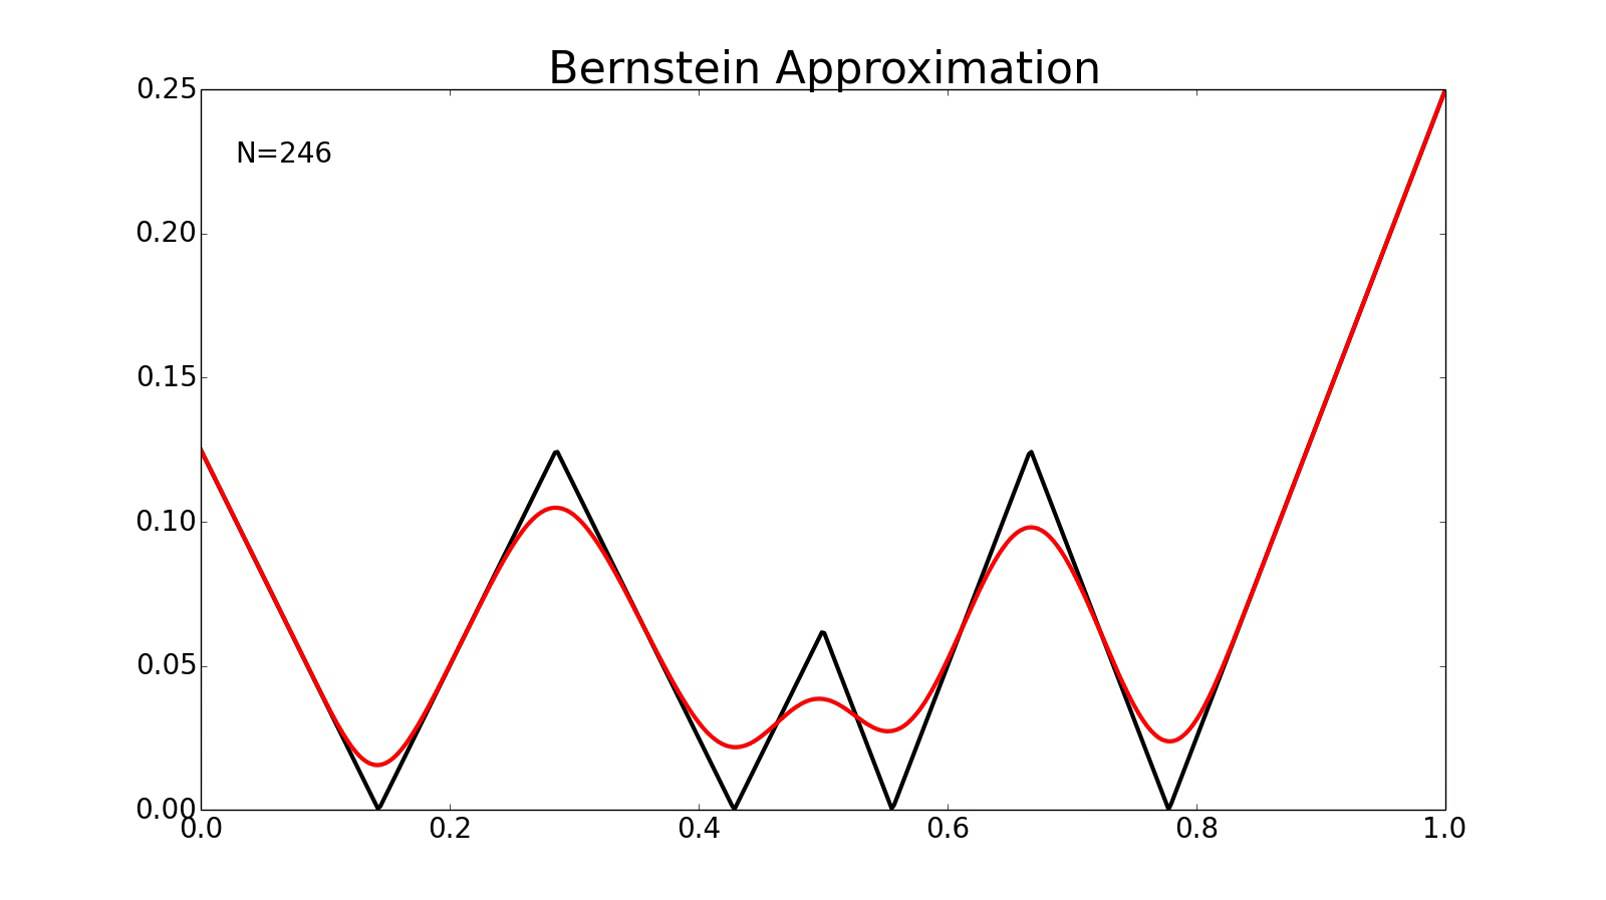
\includegraphics[height=3in]{bernstein}
\par\end{centering}
\caption{Bernstein polynomials approximating a nondifferentiable function}
\end{figure}
\begin{prop}
Let $f$ be continuous on $[0,1]$. Then, there exists a sequence
$(p_{n})_{n}$ of polynomials on $[0,1]$ such that $p_{n}\rightarrow f$
uniformly. That is,
\[
\Vert p_{n}-f\Vert_{\infty}\rightarrow0\qquad\text{as }n\rightarrow\infty.
\]
where $\Vert g\Vert_{\infty}=\sup_{x}|g(x)|$. Moreover, these polynomials,
called Bernstein polynomials, have the form
\[
p_{n}(x)=\sum_{k=0}^{n}f\left(\frac{k}{n}\right)\binom{n}{k}x^{k}\left(1-x\right)^{n-k}.
\]
\end{prop}
\begin{proof}
Let $(X_{n})_{n}$ be a sequence of i.i.d. $\operatorname{Bernoulli}(p)$
random variables, for some $0\leq p\leq1$. As usual, define $S_{n}=X_{1}+\cdots+X_{n}$.
Note that $S_{n}\sim B(n,p)$, and hence $\mathbb{E}[S_{n}]=np$ (equivalently,
$\mathbb{E}[\frac{1}{n}S_{n}]=p$). Moreover, $\operatorname{Var}(S_{n})=np(1-p)$.

By the weak law of large numbers, $S_{n}/n\rightarrow p$ in probability.
Let $\delta>0$. By Chebyshev's inequality,
\[
\mathbb{P}\left\{ \left|\frac{1}{n}S_{n}-p\right|\geq\delta\right\} \leq\frac{1}{\delta^{2}}\mathbb{E}\left[\left|\frac{1}{n}S_{n}-p\right|^{2}\right]=\frac{\operatorname{Var}(\frac{1}{n}S_{n})}{\delta^{2}}=\frac{\operatorname{Var}(S_{n})}{n^{2}\delta^{2}}=\frac{p\left(1-p\right)}{n\delta^{2}}\leq\frac{1}{4n\delta^{2}}.
\]
The last step is since 
\[
\max_{p\in[0,1]}p\left(1-p\right)=\frac{1}{4}
\]
(you can prove that by ordinary calculus: take the first derivative
and set it to zero).

Now, let $f\in C[0,1]$ be arbitrary. Since
\[
\frac{1}{n}S_{n}\rightarrow p
\]
in probability, then
\[
f\left(\frac{1}{n}S_{n}\right)\rightarrow f(p)
\]
in probability. By the dominated convergence theorem,
\[
\mathbb{E}\left[f\left(\frac{1}{n}S_{n}\right)\right]\rightarrow\mathbb{E}\left[f\left(p\right)\right].
\]
Let $\epsilon>0$. Since continuity and uniform continuity are equivalent
on compact sets, we can pick $\delta>0$ such that for $|f(x)-f(y)|<\epsilon$
whenever $|x-y|<\delta$. Therefore,
\begin{align*}
\mathbb{E}\left[\left|f\left(\frac{1}{n}S_{n}\right)-f(p)\right|\right] & \leq\epsilon\mathbb{P}\left\{ \left|\frac{1}{n}S_{n}-p\right|<\delta\right\} +2\Vert f\Vert_{\infty}\mathbb{P}\left\{ \left|\frac{1}{n}S_{n}-p\right|\geq\delta\right\} \\
 & \leq\epsilon+2\Vert f\Vert_{\infty}\frac{1}{4n\delta^{2}}.
\end{align*}
Since this bound is independent of $p$, we see $\mathbb{E}[f(S_{n}/n)]\rightarrow f(p)$
uniformly. Now, if we set $p=x$,
\[
\mathbb{E}\left[f\left(\frac{1}{n}S_{n}\right)\right]=\sum_{k=0}^{n}f\left(\frac{k}{n}\right)\binom{n}{k}x^{n}\left(1-x\right)^{n-k}.
\]
The right hand side above defines the $n$-th Bernstein polynomial,
$p_{n}(x)$.
\end{proof}

\end{document}
